\documentclass[../main/report.tex]{subfiles}
\begin{document}

\chapter{Results}

\section{Scalability of the Demolicious system}
\label{sec:scalability}

The architecture of the Demolicious system easily scales to a larger number of processors.
As there is a linear relationship between the number of streaming processors on chip and processor throughput, one can simply add more cores to increase performance.

Limiting factors to this scalability include:
\begin{enumerate}
  \item
    The more cores, the lower the clock frequency, as signal propagation time and fanout increases
  \item
    Space available on the chosen FPGA
  \item
    Power consumption constraints, as more cores increase active power consumption
\end{enumerate}

%LX45 usage
%
%8% lut, 1% slice
%
%12% lut, 2%slice fanout 4.57, 3.631 lut flipflop pairs
%
%
%28% LUT, 5% slice 8393 lut flip flop pairs
%
%
%6% Slice, 25% LUT, 36% occupied, 7958 lut flip flop pairs
%
%Not synthesizable

\todo{These numbers need regenerating. I'll do it tomorrow}
\begin{table}[H]
\begin{tabularx}{\textwidth}{cccccc}
\hline
Cores & Crit. path & Max freq. & Dynamic + quiescent power & LX16 & LX45 \\
\hline
\hline
2 / 2      & 17.103ns      & 58.469MHz & 0.272 W: 0.088 W + 0.184 W & \checkmark & \checkmark  \\
4 / 2     & 17.959ns      & 55.682MHz & 0.292 W: 0.107 W + 0.184 W & \checkmark & \checkmark \\
8 / 4   & 19.722ns      & 50.108MHz & 0.353 W: 0.168 W + 0.186 W &            & \checkmark \\
16 / 8     & X  & X & X          & \\
       &               &           &                   &    & \\
\hline
\end{tabularx}
\caption{Hardware configurations compared. Harvested from post place \& route static simulation.}
\label{table:scalability}
\end{table}

The 4-core design fits with room to spare on the LX16, but does not fit the 8-core design.
The LX45 shifts this up one notch, fitting the 8-core design, but being unable to place \& route the 16-core design.
For all processor designs, the critical path passes from the immediate field of the instruction through the ALU into the active register file.
This is something that could be increased drastically by pipelining the processor.

Figure \ref{table:scalability} shows that there is a negligible drop in maximum frequency from two to eight cores.
At 50.108MHz with 8 cores, the GPU has an instruction throughput of ~400 mips.
This compares favorably to the ~117 mips of the two-core architecture.

It does however come with a 100mAh increase in power draw.
Luckily this only constitutes a 30\% total increase in power, considerably less than the fourfold improvement in GPU throughput.
The decrease in execution time will allow both the host CPU and the GPU to enter lower power states quicker, reducing static power consumption.

\section{Performance}

In the Demolicious system, the kernel calls can be issued by the CPU in only a few cycles.
This means that the number of frames per second (FPS) that the system can display is dominated by the run time of the kernels.

\begin{figure}[H]
	\centering
	\begin{subfigure}[t]{0.45\textwidth}
		\centering
		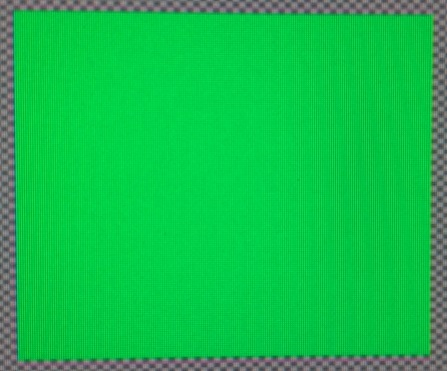
\includegraphics[width=\textwidth]{../results/diagrams/green_screen_run.jpg}
		\caption{Output from the green screen kernel.}
	\end{subfigure} 
	\begin{subfigure}[t]{0.45\textwidth}
		\centering
		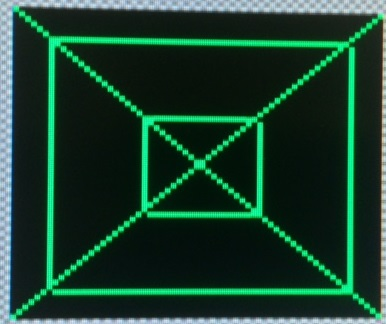
\includegraphics[width=\textwidth]{../results/diagrams/kernel_run_tunnel.jpg}	
		\caption{Output from the tunnel kernel.}
	\end{subfigure}
	\caption{Running two example kernels.}
	\label{fig:kernel_outputs}

\end{figure}

Figure \ref{fig:kernel_outputs} shows the output from the green screen kernel, and the more complex tunnel effect kernel.
It's desirable that both these kernels can be run at about 30 FPS.
Using the results presented in section \ref{sec:scalability}, the expected frames per second for varying resolutions can be estimated.

\begin{figure}[H]
	\centering
		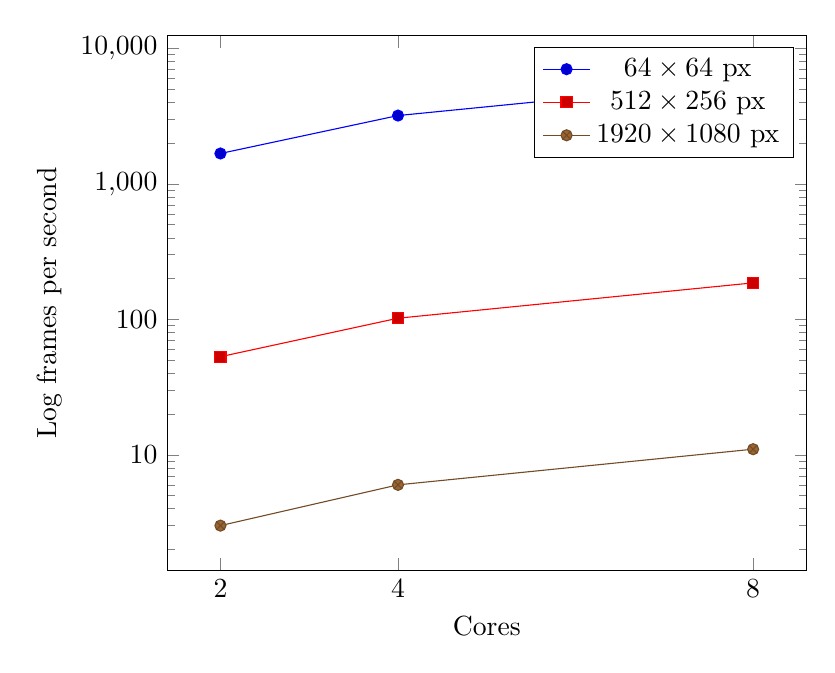
\begin{tikzpicture}
		   \begin{semilogyaxis}[
		   	   width=0.8\textwidth,
			   log ticks with fixed point,
		       xlabel=Cores,
		       ylabel=Log frames per second,
		       xtick = {2,4,8}
		   ]
				
		     \addplot plot coordinates {
		      	(2, 1678)
		      	(4, 3198)
    			(8, 5813)
		    
		  	 };
				
		   \addplot plot coordinates {
		      (2, 53)
		      (4, 102)
		      (8, 186)
		   };
		   
		   \addplot plot coordinates {
		      (2, 3)
		      (4, 6)
		      (8, 11)
		   };
		      
		   \legend{
		   $64\times64$ px \\
		   $512\times256$ px\\
		   $1920\times1080$ px\\}

		   \end{semilogyaxis}
		\end{tikzpicture}
		\caption{Running the green screen kernel.}
		\label{fig:kernel_green_screen_fps}
\end{figure}	
\begin{figure}[H]
	\centering
	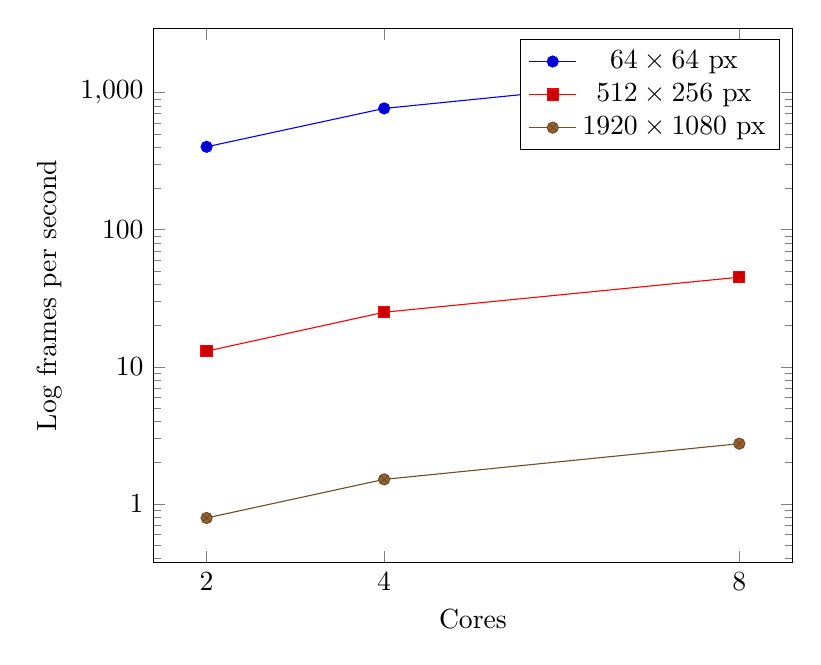
\begin{tikzpicture}
	 \begin{semilogyaxis}[
	 	 width=0.8\textwidth,
	     log ticks with fixed point,
	     xlabel=Cores,
	     ylabel=Log frames per second,
		     xtick = {2,4,8}
		 ]
		 \addplot plot coordinates {
		    (2, 402)
		    (4, 766)
		    (8, 1394)
		 };
		 \addplot plot coordinates {
		    (2, 13)
		    (4, 25 )
		    (8, 45)
		 };
		 \addplot plot coordinates {
		    (2, 0.79)
		    (4, 1.51)
		    (8, 2.75)
		 };
 
 
		 \legend{$64\times64$ px\\
		 $512\times256$ px\\
		 $1920\times1080$ px\\}

		 \end{semilogyaxis}
	\end{tikzpicture}
	\caption{Running the tunnel kernel.}	
	\label{fig:kernel_tunnel_fps}
\end{figure}


The figures \ref{fig:kernel_tunnel_fps}, and \ref{fig:kernel_green_screen_fps} display the relationship between frame rate, resolution and number of cores.
Both figures display that doubling the amount of core roughly doubles the frame rate.

For a configuration of cores, the time it takes to process one pixel is constant.
This means that the time to execute one kernel scales linearly with the resolution.
When the output resolution is increased, the amount of pixels to process increases quadratically.
As a consequence the frame rate decreases quadratically when the resolution grows.
  
For the target resolution for the project, which is $512\times256$, the project goal of maintaining 30 fps is achieved.

\section{Clock frequency}

\section{Video output}
The Demolicious system can output to a screen using HDMI.
The minimum resolution permitted by the HDMI protocol is $640\times480$,
but the size of the data memory limits the actual resolution to $512\times256$ pixels.
The rest of the screen is padded with a checker pattern.
Most of the time the output image is correct.
However, the output image is distorted under certain conditions.
\begin{figure}[H]
	\centering
	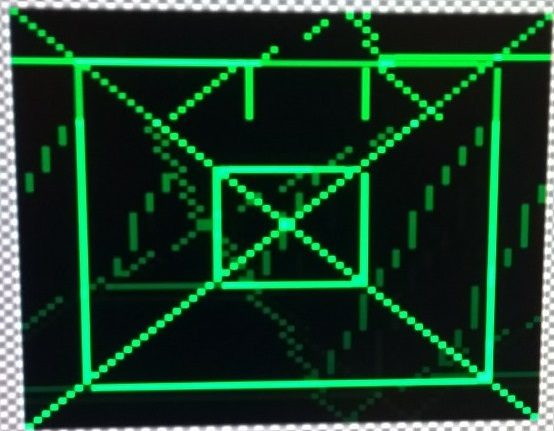
\includegraphics[width=0.8\textwidth]{../results/diagrams/flicker.jpg}
	\caption{Flickering when running the tunnel kernel. This picture was exposed over two frames.}
	\label{fig:flickering}
\end{figure}
Some kernels exhibit intermittent flickering (Figure \ref{fig:flickering}).
The exact reason for why this occurs is unclear, but
it can be observed that the flicker contains parts of the last frame. 
This may be caused by a failure in the synchronization mechanism in the video unit.

Since the GPU has priority on memory access, the video unit may get starved for data.
When the video unit is starved the buffer containing pixels to output will underflow.
For the duration of the starve, a line containing the previous pixel on the bus will be displayed on the screen.


\end{document}
